\documentclass{article}

%================================================
% パッケージの読み込み
%================================================
\usepackage{amsmath}
\usepackage{amssymb}
\usepackage{graphicx}
\usepackage{listings}
\usepackage{xcolor}
\usepackage{url}
\usepackage{array}
\usepackage{booktabs}
\usepackage{multirow}
\usepackage{subcaption}
\usepackage{float}
\usepackage{geometry}
\usepackage{tabularx}

% 日本語環境設定 (XeLaTeX用)
\usepackage{fontspec}
\usepackage{xeCJK}
\setCJKmainfont{Hiragino Sans GB}
\setCJKmonofont{Hiragino Sans GB}

%================================================
% 各種設定
%================================================

%--- ページ余白の設定 ---
\geometry{left=25mm, right=25mm, top=30mm, bottom=30mm}

%--- listings (Rコード表示) の設定 ---
\lstdefinestyle{mystyleR}{
    language=R,
    backgroundcolor=\color{white},
    commentstyle=\color{gray},
    keywordstyle=\color[rgb]{0,0,0.8},
    stringstyle=\color[rgb]{0.8,0,0},
    numberstyle=\tiny\color{gray},
    basicstyle=\ttfamily\small,
    breakatwhitespace=false,
    breaklines=true,
    captionpos=b,
    keepspaces=true,
    numbers=left,
    numbersep=5pt,
    showspaces=false,
    showstringspaces=false,
    showtabs=false,
    tabsize=2,
    frame=single,
    framesep=5pt,
    framerule=0.5pt,
}
\lstset{style=mystyleR}

%================================================
% 文書情報
%================================================
\title{データ処理・レポート}
\author{氏名:山北倫太郎 \\ 学籍番号:1423107}
\date{2025年7月6日}

%================================================
% 本文開始
%================================================
\begin{document}

\maketitle
\tableofcontents % 目次
\newpage

\section{クラスター分析とは}

クラスター分析とは、ある集団の中から、互いに性質が似ているものを集めてグループ(クラスター)に分けるための統計的な分析手法です。データに内在する構造やパターンを明らかにすることを目的とした、教師なし学習の一種です。

\subsection*{分析の手順}
一般的に、以下の手順で分析を進めます。
\begin{enumerate}
    \item \textbf{変数の選定とデータ準備:} 分析目的に合わせて変数を決定し、必要に応じて尺度を揃えるための標準化などを行います。
    \item \textbf{距離(非類似度)の計算:} 各データ点がどの程度似ていないかを定量的に示す「距離」を計算します。
    \item \textbf{クラスターの形成:} 算出した距離に基づき、データをグループ分けします。本課題で用いる階層的手法などがこれにあたります。
    \item \textbf{クラスター数の決定と結果の解釈:} 最適なクラスター数を決定し、各クラスターがどのような特徴を持つかを分析・解釈します。
\end{enumerate}

\subsection*{距離の取り方}
データ間の距離尺度には様々ありますが、本課題では\textbf{ユークリッド距離}を用います。これは、多次元空間における2点間の直線距離を示す、最も一般的な尺度です。
$$
d(p, q) = \sqrt{\sum_{i=1}^{n} (p_i - q_i)^2}
$$


\section{\texttt{USArrests}データセットの分析}

課題の指示に従い、Rに組み込まれた\texttt{USArrests}データセットの「Murder」「Assault」「UrbanPop」の3変数を用いて分析を行いました。

\subsection{(a) 階層的分類法によるクラスター分析と結論の考察}

\subsubsection*{分析方法}
\begin{itemize}
    \item \textbf{データ間の距離:} 課題の指定に基づき、\textbf{ユークリッド距離}を用いました。
    \item \textbf{クラスター間の距離:} 複数のクラスターを併合する際の手法として、\textbf{ウォード法(Ward's method)}を選択しました。ウォード法は、併合によってクラスター内の情報の損失(平方和の増加量)が最小になるようにグループを形成する手法です。
    \item \textbf{データの前処理:} 各変数は測定単位が異なるため、分析前に全変数の値を平均0、標準偏差1となるよう\textbf{標準化}を行いました。
\end{itemize}

\subsubsection*{結論と考察}
分析の結果、アメリカ50州は犯罪率と都市化の度合いに基づき、性質の異なる4つのグループに明確に分類されました。
\begin{itemize}
    \item \textbf{クラスター1(南部・殺人型):} 殺人発生率が最も高いグループ。アメリカ南部の州が多く含まれます。
    \item \textbf{クラスター2(大都市・暴行型):} 暴行発生率が突出して高く、都市人口比率も高いグループ。大都市を抱える州が多く見られます。
    \item \textbf{クラスター3(全米平均型):} 各指標が全米の平均値に近く、標準的な特徴を持つグループ。
    \item \textbf{クラスター4(地方・平和型):} 殺人・暴行発生率が共に著しく低く、最も安全な州のグループ。
\end{itemize}
この結果から、各州の治安状況は単に「良い・悪い」だけでは測れず、「どのような犯罪が多いか」という質的な違いが存在することが示唆されます。クラスター分析を用いることで、こうしたデータに隠れた複雑な構造を客観的に明らかにすることができました。


\subsection{(b) デンドログラムの作成}
階層的クラスター分析の結果を可視化するために、以下のプログラムを用いてデンドログラム(樹形図)を作成しました。

\subsubsection*{プログラム}
\begin{lstlisting}[language=R, caption=デンドログラム作成用Rコード]
# データの準備(読み込み、変数選択、標準化)
library(clustrd)
data(USArrests)
USArrests_selected <- USArrests[, c("Murder", "Assault", "UrbanPop")]
USArrests_scaled <- scale(USArrests_selected)

# 距離行列の計算とクラスタリングの実行
d <- dist(USArrests_scaled, method = "euclidean")
hc <- hclust(d, method = "ward.D2")

# デンドログラムの描画
plot(hc, hang = -1, cex = 0.6, main = "Dendrogram of USArrests")
rect.hclust(hc, k = 4, border = "red") 
\end{lstlisting}

\subsubsection*{作成されたデンドログラム}
\begin{figure}[H]
    \centering
    % !!以下のパスはご自身の環境に合わせて修正してください!!
    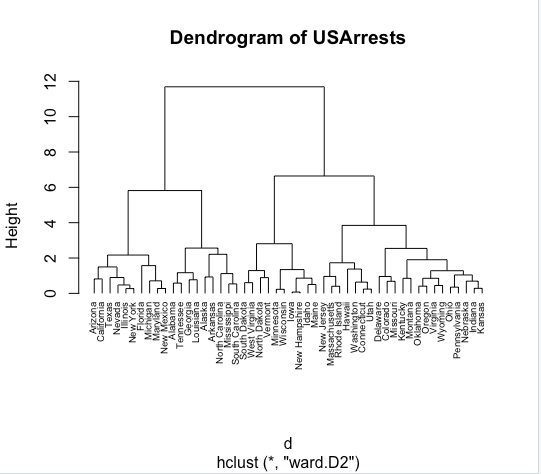
\includegraphics[width=\textwidth]{/Users/rintaro/Downloads/Github_private/machine_learning/cluster_analysis/pic1.png}
    \caption{USArrestsデータセットのデンドログラム}
    \label{fig:dendrogram}
\end{figure}


\subsection{(c) クラスター数4の場合の所属州と使用プログラム}
クラスターの数を4つとした場合に、どの州がどのクラスターに属するかを調べるためのプログラムと、その実行結果を以下に示します。

\subsubsection*{プログラム}
\begin{lstlisting}[language=R, caption=クラスター所属特定用Rコード]
# (b)で実行したクラスタリング結果(hc)を4つのクラスターに分割
clusters <- cutree(hc, k = 4)

# クラスター番号ごとに州の名前を一覧表示する
for (i in 1:4) {
  cat("Cluster", i, ":\n")
  print(names(clusters[clusters == i]))
  cat("\n")
}
\end{lstlisting}

\subsubsection*{各クラスターの所属州}
\begin{table}[H]
    \centering
    \caption{クラスター分類結果}
    \label{tab:clusters}
    \begin{tabularx}{\textwidth}{|l|X|}
        \hline
        \textbf{クラスター番号} & \textbf{所属する州} \\
        \hline
        \textbf{Cluster 1} & Alabama, Arkansas, Georgia, Louisiana, Mississippi, North Carolina, South Carolina, Tennessee \\
        \hline
        \textbf{Cluster 2} & Alaska, Arizona, California, Florida, Illinois, Maryland, Michigan, Nevada, New Mexico, New York, Texas \\
        \hline
        \textbf{Cluster 3} & Colorado, Connecticut, Delaware, Hawaii, Indiana, Kansas, Kentucky, Massachusetts, Missouri, Montana, Nebraska, New Jersey, Ohio, Oklahoma, Oregon, Pennsylvania, Rhode Island, Utah, Virginia, Washington, Wyoming \\
        \hline
        \textbf{Cluster 4} & Idaho, Iowa, Maine, Minnesota, New Hampshire, North Dakota, South Dakota, Vermont, West Virginia, Wisconsin \\
        \hline
    \end{tabularx}
\end{table}


\section{分析の感想}
今回の分析を通して、一見するとただの数値の羅列である統計データから、クラスター分析という手法を用いることで、意味のあるパターンや構造を浮かび上がらせることができる点を実感しました。特に、事前に何の正解も与えていないにもかかわらず、アメリカの州が我々の持つ地理的なイメージ(例えば「南部」や「大都市圏」)に近い形で自然にグループ分けされたことには、純粋な驚きがありました。

また、「犯罪率が高い」という単純な括りの中でも、殺人が多い「クラスター1」と暴行が多い「クラスター2」のように、その内実が異なるグループが形成されたことは、データ分析の奥深さを示しているように感じます。今回の分析は3つの変数のみで行いましたが、ここに所得水準や失業率、教育レベルといった新たな変数を加えることで、また違った側面から各州の姿が見えてくるのではないかと、さらなる分析への興味が湧きました。

\section{参考文献}
\begin{thebibliography}{9}
    \item 山田 剛史, 杉澤 正人 (2019). \textit{Rによる多変量解析}. 株式会社オーム社.
    \item 脇本 和昌 (2014). \textit{多変量解析入門}. 株式会社朝倉書店.
\end{thebibliography}

\end{document}